\section*{Kinetics, Constitutive Laws, and Viscoelasticity I}

\subsection*{2--1. \textbf{Balance of mass} [4 pts].} 
A large piece of polydimethylsiloxane (PDMS) of uniform density $\rho(\bm{x},t)$ has a central spherical bubble of time-evolving radius $R(t)$, initial radius $R_0$, and wall velocity of $\dot{R}$. 
The hole is subject to a uniform surface traction in the $\bm{e}^{(r)} \equiv \bm{e}_{\bm{r}}$ direction from an axisymmetric pressure, and maintains spherical symmetry over time. 

\medskip
The position of a point in the material can be written as $\bm{x} = r(R,t) \bm{e}_{\bm{r}}$ with reference position $\bm{X} = r_0(R_0)$, while the velocity of that point can be written as $\bm{v}(r,t) = v_r \bm{e}_{\bm{r}}$.

\medskip
Using the conservation of mass equation, show that the material must satisfy
%\begin{equation}
%\rho_{,t} + (\rho v_i)_{,i} = 0,
%\end{equation}
\begin{equation*}
\rho_{,t}+ \rho_{,r} v_r + \frac{\rho}{r} (\textcolor{red}{2}v_r + r v_{r,r}) = 0,
\end{equation*}
and hence, show that an assumption of incompressibility for PDMS results in 
\begin{equation*}
v_r(r,t) = \frac{R^2 \dot{R}}{r^2}.
\end{equation*}

\textbf{Solution:}

We know that the conservation of mass is defined as
\begin{equation*}
    \frac{\partial \rho}{\partial t} + \frac{\partial}{\partial x_i} (\rho v_i) = \frac{\partial \rho}{\partial t} + \frac{\partial \rho}{\partial x_i}v_i + \rho \frac{\partial v_i}{\partial x_i} = 0
\end{equation*}
We now need to convert this equation from Cartesian to spherical $\{ r, \theta, \phi\}$ coordinates:

\begin{equation*}
    \frac{\partial \rho}{\partial t} + \left(\frac{\partial \rho}{\partial r}\bm{\hat{r}} + \frac{1}{r} \frac{\partial \rho}{\partial \theta} \bm{\hat{\theta}} + \frac{1}{r\sin(\theta)}\frac{\partial \rho}{\partial \phi} \bm{\hat{\phi}}\right) \cdot (v_r\bm{\hat{r}}) + \rho \left(\frac{\partial v_r}{\partial r} + \frac{2}{r} v_r\right) = 0.
\end{equation*}

It should be noted that the last section of that equation is given in Bower, as the divergence of a vector function in spherical coordinates, with $v_\theta$ and $v_\phi$ ignored because we're only dealing with $v_r$ in this case. We can also simplify the equation above due to the fact that the dot product of the terms in the $\hat{\theta}$ and $\hat{\phi}$ directions will result in zero when dotted with the $\hat{r}$ direction. This leaves us with:

\begin{equation*}
    \frac{\partial \rho}{\partial t} + \frac{\partial \rho}{\partial r} v_r + \rho \frac{\partial v_r}{\partial r} + \frac{2\rho}{r}v_r = 0.
\end{equation*}

Thanks to the assumption of incompressibility, we can cancel the first two terms to zero since the density can be assumed constant. This finally leaves us with an expression that enables to solve for the final result:
\begin{align*}
    \rho \frac{\partial v_r}{\partial r} &= -\frac{2\rho}{r}v_r\\
    \int_{\dot R}^{v_r} \frac{1}{v_r} \textrm{d}v_r &= -2 \int_R^r \frac{1}{r} \textrm{d}r\\
    \ln\left(\frac{v_r}{\dot R}\right) &= 2\ln\left(\frac{R}{r}\right)\\
    \ln\left(\frac{v_r}{\dot R}\right) &= \ln \left(\frac{R}{r}\right)^2\\
    v_r(r,t) &= \frac{R^2 \dot R}{r}.
\end{align*}

\medskip
\newpage
\subsection*{2--2. \textbf{Balance of momenta} [4 pts].} A spherical hydrogel body $\mathcal{B}$ with a linear density gradient is currently submerged in water as depicted in the figure. 
The sphere has coordinates $\bm{x}$ in a region $\Omega$ with position-dependent density $\rho(\bm{x})$. 

\begin{figure}[H]
\vspace{-2em}
\centering
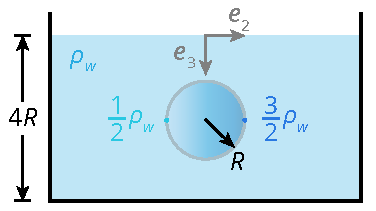
\includegraphics[width=3in]{instr-figures/PS2-Q1.pdf}
\caption{\small{Hydrogel sphere with a linear density gradient submerged in water. The water has a density $\rho_w$, while the sphere has a density at its leftmost point of $\rho_w/2$ and at its rightmost point of $3\rho_w/2$.}}
\end{figure}

\vspace{-1em}
The surface traction $\bm{t}(\bm{x},\hat{\bm{n}})$ acting on $\mathcal{B}$ is given by 
\begin{equation*}
\bm{t}(\bm{x},\hat{\bm{n}}) = -\rho_w g x_3 \hat{\bm{n}},
\end{equation*}
where $\hat{\bm{n}}$ is the outer unit normal to the surface $\partial \Omega_t$ and $\rho_w$ is the (constant) density of water and $g$ is the acceleration due to gravity. 

\medskip
(a) Determine the net force and moment acting on $\mathcal{B}$ via volume integrals.

\medskip
(b) Under what \textit{two} conditions is $\mathcal{B}$ in static equilibrium?

\textbf{Solution:}

\textbf{(a)}

To calculate the traction force, we integrate the surface traction over the area of the hydrogel body:

\begin{align*}
    \int_{\partial \Omega_t} \bm{t}(\bm{x}, \bm{\hat{n}}) \textrm{d}A_{\bm{x}} &= \int_{\partial \Omega_t} -\rho_w g x_3 \bm{\hat{n}} \textrm{d}A_{\bm{x}} = g \int_{\Omega_t} \nabla_{\bm{x}} \cdot (-\rho_w x_3) \bm{I} \textrm{d}V_{\bm{x}}\\
    &= g \int_{\Omega_t} \frac{\partial}{\partial x_3} (-\rho_w x_3) \textrm{d}V_{\bm{x}} = -g \int_{\Omega_t} \rho_w \textrm{d}V_{\bm{x}} \bm{\hat{e}_3}\\
    &= -\rho_w g \Omega_t \bm{\hat{e}_3}.
\end{align*}

To calculate the body force, we repeat the same procedure but for the body force:

\begin{equation*}
    \int_{\Omega_t} \bm{b} \textrm{d}V_{\bm{x}} = \int_{\Omega_t} \rho(\bm{x}, t) g \bm{\hat{e}_3} \textrm{d}V_{\bm{x}} = \textrm{Mass}(\mathcal{B}) g \bm{\hat{e}_3}.
\end{equation*}

Now we know that the net force will be equal to the sum of the traction force and the body force. Both are fairly straightforward as the volume is a pure calculation of the volume of the sphere. And since the gradient of the density is linear, we can simply average the two extremes of the densities to obtain the average density for body $\mathcal{B}$. I verified this by actually evaluating the triple integral, but will not show that work here.

\begin{equation*}
    \mathrm{Mass} (\mathcal{B})g \bm{\hat{e}_3} = \frac{4\pi R^3}{3}\rho_w g \bm{\hat{e}_3}.
\end{equation*}

The net force acting on $\mathcal{B}$ is thus 0.

We can also define the function for the density in the body in spherical coordinates as
\begin{equation*}
    \rho(\phi) = \rho_w (1+ \frac{r}{2R}\cos(\phi)),
\end{equation*}
where $\phi$ is the angle in the $\e{2}$-$\e{3}$ plane, going from $\phi=0$ at the rightmost point of the hydrogel counter-clockwise to $\phi=\pi$ at the leftmost point of the hydrogel.

For the net moment, we have to compute the moments due to tractions and due to body forces. For the moment due to tractions:

\begin{align*}
\int_{\partial \Omega_t} \bm{x} \times \bm{t}(\bm{x}, \bm{\hat{n}}) \mathrm{d}A_{\bm{x}} &=  \int_{\partial \Omega_t} \bm{x} \times \bm{\hat{n}} \cdot \bm{\sigma} \mathrm{d}A_{\bm{x}} \rightarrow  \int_{\partial \Omega_t} \epsilon_{ijk} x_j \sigma_{mk} \hat{n}_m \mathrm{d}A_{\bm{x}}\\
&= \int_{\Omega_t} \epsilon_{ijk} \frac{\partial}{\partial x_m} (x_j \sigma_{mk}) \bm{\hat{e}_i} \mathrm{d}V_{\bm{x}}\\
&= -\rho_w g \int_{\Omega_t} \epsilon_{ijk} \frac{\partial}{\partial x_m} (x_j x_3 \delta_{mk}) \bm{\hat{e}_i} \mathrm{d}V_{\bm{x}}\\
&= -\rho_w g \int_{\Omega_t} \epsilon_{ijk} \frac{\partial}{\partial x_k} (x_j x_3) \bm{\hat{e}_i} \mathrm{d}V_{\bm{x}}\\
&= -\rho_w g \int_{\Omega_t} \epsilon_{ijk} (\delta_{jk} x_3 + x_j \delta_{3k}) \bm{\hat{e}_i} \mathrm{d}V_{\bm{x}}\\
&= -\rho_w g \int_{\Omega_t} (x_2 \bm{\hat{e}_1} - x_1 \bm{\hat{e}_2}) \mathrm{d}V_{\bm{x}}\\
&= -2\rho_w g \int_0^\pi \int_0^{2\pi} \int _0^R (r\cos(\phi)\bm{\hat{e}_1} - r\sin(\phi)\cos(\theta)\bm{\hat{e}_2}) r^2 \sin(\phi) \mathrm{d}r \mathrm{d}\theta \mathrm{d}\phi\\
&= -2\rho_w g \int_0^\pi \int_0^{2\pi} \left[ \frac{R^4}{4} \sin(\phi)\cos(\phi)\bm{\hat{e}_1} - \frac{R^4}{4}\sin^2 (\phi) \cos(\theta)\bm{\hat{e}_2}\right] \mathrm{d}\theta \mathrm{d}\phi\\
&= -2\rho_w g \int_0^\pi \left[ \frac{\pi R^4}{2} \sin(\phi)\cos(\phi) \bm{\hat{e}_1} \right] \mathrm{d}\phi\\
&= -2\rho_w g \left[ \frac{\pi R^4}{2} \sin^2(\phi) |_0^{\pi} \bm{\hat{e}_1} \right] = 0.
\end{align*}

For the body moment, we follow basically the same procedure:

\begin{align*}
    \int_{\Omega_t} \bm{x} \times \bm{b} \dd V_{\bm{x}} &= \int_{\Omega_t} \bm{x} \times \rho(\bm{x},t) g \e{3} \dd V_{\bm{x}} \rightarrow \int_{\Omega_t} \rho(\bm{x},t) g \epsilon_{ij3} x_j \e{3} \e{i} \dd V_{\bm{x}}\\
    &= \int_{\Omega_t} \rho(\bm{x}, t) g (x_2 \e{1} - x_1 \e{2}) \dd V_{\bm{x}}\\
    &= 2\rho_w g \int_0^{\pi} \int_0^{2\pi} \int_0^{R} (1+\frac{r}{2R}\cos(\phi))(r\cos(\phi)\e{1} - r\sin(\phi)\cos(\theta)\e{2}) r^2 \sin(\phi) \dd r \dd \theta \dd \phi\\
    &= 2 \rho_w g \int_0^{\pi} \int_0^{2\pi} \left[ \left( \frac{R^4}{4}\cos(\phi)\sin(\phi) + \frac{R^4}{10}\cos^2 (\phi)\sin(\phi)\right) \e{1}\\
    &-\left \left( \frac{R^4}{4}\sin^2 (\phi) \cos(\theta) + \frac{R^4}{10}\sin(\phi)\cos(\phi)\cos(\theta) \right) \e{2} \right] \dd \theta \dd \phi\\
    &= 2\rho_w \int_0^{\pi} \left[ 2\pi \left( \frac{R^4}{4}\cos(\phi)\sin(\phi) + \frac{R^4}{10}\cos^2(\phi)\sin(\phi) \right) \e{1} \right] \dd \phi\\
    &= 2\rho_w g \left[ 2\pi \left( \frac{R^4}{8}\sin^2(\phi) |_0^{\pi} - \frac{R^4}{30}\cos^3 (\phi) |_0^{\pi}  \right)\right]\\
    &= \frac{4\pi\rho_w g R^4}{30} \e{1}.
\end{align*}

The net moment is therefore simply equal to the body moment.

\textbf{(b)}

$\mathcal{B}$ is in static equilibrium under the condition of the net force and net moment acting on the body both being zero. The net force is already zero, meaning that the hydrogel is naturally buoyant, so that condition is satisfied. The net moment, however, is nonzero. This makes sense because, due to the linear density gradient, the center of mass is not in the center of the spherical hydrogel, but rather at 2/3 of the width of the hydrogel to the right. Therefore, in order to satisfy the body being in static equilibrium, we need to rotate the body by 90$^{\circ}$ clockwise, for the center of mass to be at the lowest possible point.

\newpage
\bigskip
\subsection*{2--3. \textbf{Viscoelastic data} [4 pts].} 
Stress relaxation isochrones for a compliant viscoelastic material are shown in the figure below.  

\begin{figure}[H]
\vspace{-1em}
\centering
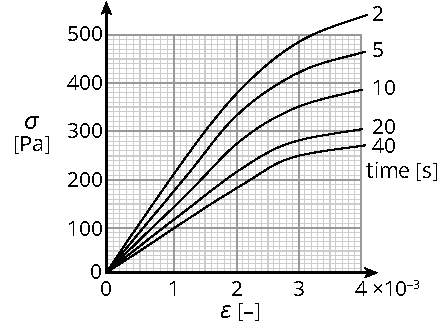
\includegraphics[scale = 1.5]{instr-figures/PS2-Q3.pdf}
\caption{\small{Stress (Pa) vs. strain ($-$) for a soft viscoelastic material.}}
\end{figure}

\vspace{-1em}
(a) Are these isochrones from a material which we can describe with linear viscoelasticity? If not, why not, and if so, under what approximate regimes would this assumption be valid? 

\medskip
(b) Estimate the creep relaxation function $J_c$ for stress values of 100 and 250 Pa. Isochrones are shown at times of 2, 5, 10, 20, and 40 seconds.   

\textbf{Solution:}

\textbf{(a)}

These isochrones seem to be from a material that can be described as linear viscoelastic for strains up to about 1.5. Past that, we can see that the curves start becoming non-linear and thus don't follow LVE anymore. We can therefore say that this material can be represented as linear viscoelastic for small strains (below strains of 1.5).

\textbf{(b)}

To estimate the creep relaxation function $J_c$ for these two stress values, I first have to read off data from the graph and then compute the value of $J_c$ for each of the two stress levels at each of the five times.
\newpage
The table with calculations for 100 Pa can be seen below in Table \ref{100Pa}:

\begin{table}[h!]
\centering
\caption{$J_c$ values for five of the measured times at 100 Pa}
\begin{tabular}{ccccc} \label{100Pa}
\textbf{Time (s)} & $\bm{\varepsilon}$ & $\mathbf{E(t) = \bm{\sigma} / \bm{\varepsilon}}$ \textbf{(Pa)} & $\mathbf{J_c (t) = 1/E(t)}$ \textbf{(1/Pa)} & $\mathbf{J_c (t) / 100} \,\textbf{Pa}$ \textbf{(1/Pa$\mathbf{^2}$)} \\
\hline\hline
2  & 0.43 & 232.56 & 0.0043 & 0.000043 \\
5  & 0.52 & 192.31 & 0.0052 & 0.000052 \\
10 & 0.66 & 151.52 & 0.0066 & 0.000066 \\
20 & 0.81 & 123.46 & 0.0081 & 0.000081 \\
40 & 1.00 & 100.00 & 0.0100 & 0.000100 \\
\end{tabular}
\end{table}

And the table with calculations for 250 Pa can be see in Table \ref{250Pa}:

\begin{table}[h!]
\centering
\caption{$J_c$ values for five of the measured times at 250 Pa}
\begin{tabular}{ccccc} \label{250Pa}
\textbf{Time (s)} & $\bm{\varepsilon}$ & $\mathbf{E(t) = \bm{\sigma} / \bm{\varepsilon}}$ \textbf{(Pa)} & $\mathbf{J_c (t) = 1/E(t)}$ \textbf{(1/Pa)} & $\mathbf{J_c (t) / 250} \,\textbf{Pa}$ \textbf{(1/Pa$\mathbf{^2}$)} \\
\hline\hline
2  & 1.20 & 208.33 & 0.0048 & 0.0000192 \\
5  & 1.45 & 172.41 & 0.0058 & 0.0000232 \\
10 & 1.80 & 138.89 & 0.0072 & 0.0000288 \\
20 & 2.40 & 104.17 & 0.0096 & 0.0000384 \\
40 & 3.00 & 83.33  & 0.0120 & 0.0000480 \\
\end{tabular}
\end{table}

The last columns of these tables, which show the normalized creep relaxation time for stress are quite different between the two stresses. That suggests that this is not very accurately modeled by LVE because if it was, the $J_c (t,\sigma) / \sigma$ vs. $\sigma$ would be flat, but here, the values between the two stresses, vary in multiples of each other.

\newpage
\bigskip
\subsection*{2--4. \textbf{Impulsive stresses} [4 pts].}

(a) Say that instead of a step load, we apply $\sigma(t) = A \delta(t)$ to an unknown linear viscoelastic material. 
Determine the strain history $\epsilon(t)$, first as a general function of the creep relaxation function $J_c(t)$, and then for a Kelvin-Voigt solid. 

(b) Now, consider a rapid load followed by a rapid reverse load by applying a doublet function of stress, i.e. $\sigma(t) = B \psi(t)$. 
What is the strain function $\epsilon(t)$ in terms of $J_c(t)$ and for a Kelvin-Voigt material now?

\textbf{Solution:}

\textbf{(a)}

To determine the strain history as a general function, we can utilize Laplace transforms:

\begin{align*}
    \varepsilon (t) &= \int_0^t J_c (t-\tau) \frac{\textrm{d} \sigma (\tau)}{\textrm{d} \tau} \textrm{d}\tau\\
    \varepsilon (s) &= \mathcal{L} \left\{ \int_0^t J_c (t-\tau) \frac{\textrm{d} \sigma (\tau)}{\textrm{d} \tau} \textrm{d}\tau \right\}\\
    &= \mathcal{L} \{ J_c (t)\} \mathcal{L} \left \{ \frac{\textrm{d}\sigma (t)}{\textrm{d} \tau}\right\}\\
    &= J_c (s) \cdot sA\\
    \varepsilon (s) &= sAJ_c(s)\\
    \varepsilon (t) &= A \frac{\mathrm{d}}{\mathrm{d}t} (J_c(t)).
\end{align*}

For a Kelvin-Voigt material, then, we just have to utilize the definition of the creep relaxation function $J_c (t) = \frac{1}{E} (1 - e^{-Et/\eta})$.

Since

\begin{equation*}
    \frac{\mathrm{d}}{\mathrm{d}t} (J_c(t)) = \frac{E}{\eta E} e^{- Et/\eta} = \frac{1}{\eta} e^{-Et/\eta},
\end{equation*}

the strain history for a Kelvin-Voigt material in this case will be

\begin{equation*}
    \varepsilon (t) = \frac{A}{\eta} e^{-Et/\eta}.
\end{equation*}

\textbf{(b)}

Now, with $\sigma(t) = B\psi(t)$, we follow the same procedure to obtain the general function.

\begin{align*}
    \varepsilon (s) &= \mathcal{L} \left\{ \int_0^t J_c (t-\tau) \frac{\textrm{d} \sigma (\tau)}{\textrm{d} \tau} \textrm{d}\tau \right\}\\
    &= J_c (s) \mathcal{L} \left \{ \frac{B \mathrm{d} (\psi (t))}{\mathrm{d}t} \right \}\\
    \varepsilon (s) &= B s^2 J_c (s)\\
    \varepsilon (t) &= B \frac{\mathrm{d}^2}{\mathrm{d}t^2} (J_c(t)).
\end{align*}

And then, by calculating the second derivative of the creep relaxation function, we obtain what the strain history looks like for a Kelvin-Voigt material when subjected to a doublet function of stress.

\begin{equation*}
    \varepsilon (t) = -\frac{BE}{\eta ^2} e^{-Et/\eta}.
\end{equation*}

\bigskip
\newpage
\subsection*{2--5. \textbf{Two-element models} [8 pts].}

Dynamic mechanical analysis (DMA) is a common technique for characterizing viscoelasticity. 
DMA conventionally involves application of a sinusoidal displacement to the top surface of a sample at a controllable temperature. 
Often, the user puts the sample into initial compression, and follows with the sinusoidal profile. 
A cylindrical sample of height $h$ and diameter $d$ is placed between two plates.
The DMA then quickly puts the sample into compression by moving its top plate downward by a displacement $d$, and then oscillates sinusoidally between positions $0$ and $2d$ at a frequency $\omega$.

\medskip
(a) Using the constitutive law for a Kelvin-Voigt material, determine the stress $\sigma(t)$ exerted by the platens to cause the applied strain. 

\medskip
(b) The resulting stress lags behind the strain by an phase $\delta$, as in $\sin(\omega t + \delta)$. 
Commonly this is reported as the ``tangent loss", or $\tan\delta$, for a material. 
What is the value of $\tan\delta$ for this particular Kelvin-Voigt model?

\medskip
(c) Say instead of prescribing the strain $\epsilon(t)$, we instead prescribed the stress, $\sigma(t) = - \sigma_0 - \sigma_0 \sin(\omega t)$. 
Determine the strain $\epsilon(t)$ for this prescribed stress.

\medskip
(d) Prove that the tangent loss function $\tan\delta$ is identical between the two loading methods.

\textbf{Solution:}

\textbf{(a)}

The initial strain here is $\varepsilon_0 = d/h$. Since it then goes sinusoidally between 0 and $2d$ at a frequency of $\omega$, we can define the strain as
\begin{equation*}
    \varepsilon(t) = \varepsilon_0 (1 + \sin(\omega t)).
\end{equation*}

Then we can relate this to stress through
\begin{align*}
    \sigma (t) &= \eta \dot \varepsilon (t) + E \varepsilon (t)\\
    &= \eta \omega \epsilon_0 \cos (\omega t) + E\varepsilon_0 (1 + \sin(\omega t)).
\end{align*}

\textbf{(b)}

Since we only care about the oscillatory part of $\sigma(t)$ we can define

\begin{equation*}
    \sigma_{\mathrm{osc}} (t) = \varepsilon_0 ( E \sin(\omega t) + \eta \omega \cos(\omega t)).
\end{equation*}

Now we can utilize this trigonometric identity:

\begin{equation*}
    R \sin (\omega t + \delta) = R\sin(\omega t)\cos(\delta) + R\cos(\omega t)sin(\delta).
\end{equation*}

Now we can compare the identity with the equation we have defined for $\sigma_{\mathrm{osc}} (t)$.

\begin{align*}
    E &= R\cos(\delta)\\
    \eta \omega &= R\sin(\delta),
\end{align*}

from which we can then derive:

\begin{align*}
    R &= \sqrt{E^2 (\eta \omega)^2}\\
    \tan(\delta) &= \frac{\eta \omega}{E}.
\end{align*}

\textbf{(c)}

With the stress defined, we can equate it to strain like so:

\begin{equation*}
    -\sigma_0 (1 + \sin(\omega t)) = \eta \dot \varepsilon (t) + E \varepsilon (t).
\end{equation*}

This is a first-order linear differential equation, which we can solve in a fairly straightforward manner.

To start, the homogeneous solution is simply the solution to
\begin{equation*}
    \dot \varepsilon + \frac{E}{\eta} \varepsilon(t) = 0,
\end{equation*}
which is
\begin{equation*}
    \varepsilon_h (t) = C e^{-Et/\eta},
\end{equation*}
where $C$ is just an arbitrary constant.

For the particular solution, we can start with the constant term, which will simply yield
\begin{equation*}
    \varepsilon_{\mathrm{const}} = \frac{-\sigma_0}{E}.
\end{equation*}

For the harmonic part of the particular solution, we can define a trial solution as
\begin{align*}
    \varepsilon_{\mathrm{harm}} (t) &= A\sin(\omega t) + B\cos(\omega t)\\
    \dot \varepsilon_{\mathrm{harm}} (t) &= A\omega\cos(\omega t) - B\omega\sin(\omega t).
\end{align*}

Plugging these trial functions into the expression at the start of section (c), we get
\begin{equation*}
    \eta A \omega \cos(\omega t) - \eta B \omega \sin(\omega t) + EA\sin(\omega t) + EB\cos(\omega t) = -\sigma_0 \sin(\omega t).
\end{equation*}

Now, by matching terms, we get
\begin{align*}
    \eta A \omega + EB &= 0\\
    EA - \eta B \omega &= -\sigma_0,
\end{align*}
 from which, by some mathematical manipulation, we can obtain the solutions to A and B as
 \begin{align*}
     A &= \frac{-\sigma_0 E}{E^2 + (\eta \omega)^2}\\
     B &= \frac{\eta \sigma_0 \omega}{E^2 + (\eta \omega)^2}.
 \end{align*}

 Therefore, the final expression for strain is
 \begin{equation*}
     \varepsilon(t) = -\frac{\sigma_0}{E} + \left[ \frac{-\sigma_0 E}{E^2 + (\eta \omega)^2} \sin(\omega t) + \frac{\sigma_0 \eta \omega}{E^2 + (\eta \omega)^2} \cos(\omega t) \right] + Ce^{-Et/\eta}.
 \end{equation*}

 \textbf{(d)}
 
 For this part, the important part of the strain equation is the part in the square brackets, which is the harmonic part. Again, as before, we can compare the terms here to $R$ and $\delta$.

 \begin{align*}
     \frac{-\sigma_0 E}{E^2 + (\eta \omega)^2} &= R\cos(\delta)\\
     \frac{\sigma_0 \eta \omega}{E^2 + (\eta \omega)^2} &= R\sin(\delta).
 \end{align*}
 Solving this system of equations yields
 \begin{align*}
     R &= \frac{\sigma_0}{\sqrt{E^2 (\eta \omega)^2}}\\
     \tan (\delta) = -\frac{\eta \omega}{E}.
 \end{align*}

 This shows that the magnitude of the tangent loss function is identical between the two loading methods.
 
